\documentclass[a4paper]{article}
\usepackage[UTF8]{ctex}
\usepackage{tikz}\usetikzlibrary{arrows,calc,intersections,through,backgrounds,math,angles,shapes}
\usepackage{hyperref}
\usepackage{amsmath,amssymb,mathrsfs}
\usepackage[includemp=true,marginparsep=.5cm,marginparwidth=3cm,left=2.5cm,right=2cm]{geometry}%带旁注
\def\sky{\par\vspace*{1ex}}
\newcommand\tbs[1][]{\tt\char`\\#1}
\newcommand\Dd{\displaystyle}
\newcommand\bpics[1]{\par\vspace{1ex}\noindent\begin{minipage}{\textwidth}\begin{minipage}{#1\textwidth}}
\newcommand\mpics[1]{\end{minipage}\begin{minipage}{#1\textwidth}\linespread{1}}
\newcommand\epics{\end{minipage}\end{minipage}\par\vspace{2ex}}
  \newcommand\abc[1]{\textcolor{black}{$#1$}}\def\A{\abc{A}}\def\B{\abc{B}}\def\C{\abc{C}}\def\D{\abc{D}}\def\E{\abc{E}}\def\F{\abc{F}}\def\G{\abc{G}}\def\H{\abc{H}}\def\I{\abc{I}}\def\J{\abc{J}}\def\K{\abc{K}}\def\L{\abc{L}}\def\M{\abc{M}}\def\N{\abc{N}}\def\O{\abc{O}}\def\P{\abc{P}}\def\Q{\abc{Q}}\def\R{\abc{R}}\def\S{\abc{S}}\def\T{\abc{T}}\def\U{\abc{U}}\def\V{\abc{V}}\def\W{\abc{W}}\def\X{\abc{X}}\def\Y{\abc{Y}}\def\Z{\abc{Z}}
  \def\sky{\vspace*{1ex}}
  \newcommand\beginp[1]{\tbs{begin}\{#1\}}
  \newcommand\pend[1]{\tbs{end}\{#1\}}
\begin{document}
\tableofcontents
\section{快速参考}
  \subsection{线型}
    \begin{tikzpicture}
      %线型
        \draw[solid](0,3)--(1,3) node[right=1em]{solid:默认};
        \draw[dotted](0,2.5)--(1,2.5) node[right=1em]{dotted};
        \draw[densely dotted](0,2)--(1,2) node[right=1em]{densely dotted};
        \draw[loosely dotted](0,1.5)--(1,1.5) node[right=1em]{loosely dotted};
        \draw[dashed](0,1)--(1,1) node[right=1em]{dashed};
        \draw[densely dashed](0,0.5)--(1,0.5) node[right=1em]{densely dashed};
        \draw[loosely dashed](0,0)--(1,0) node[right=1em]{loosely dashed};
        \draw[double](0,-.5)--(1,-.5) node[right=1em]{double};

      %线的粗细
        \draw[ultra thin](5,3)--(6,3)node[right=1em]{ultra thin\quad0.1pt};
        \draw[very thin](5,2.5)--(6,2.5)node[right=1em]{very thin\quad0.2pt};
        \draw[thin](5,2)--(6,2)node[right=1em]{thin\quad0.4pt};
        \draw[semithick](5,1.5)--(6,1.5)node[right=1em]{semithick\quad0.6pt};
        \draw[thick](5,1)--(6,1)node[right=1em]{thick\quad0.8pt};
        \draw[very thick](5,.5)--(6,.5)node[right=1em]{very thick\quad1.2pt};
        \draw[ultra thick](5,0)--(6,0)node[right=1em]{ultra thick\quad1.6pt};
        \draw(5,-0.5)(5.1,-0.5)node[right]{也可以通过 line width 直接定义};
      %箭头
        \draw[->](10,3)--(11,3)node[right=1em]{to};
        \draw[-latex](10,2.5)--(11,2.5)node[right=1em]{latex};
        \draw[->>,>=stealth](10,2)--(11,2)node[right=1em]{stealth};
        \draw[|-|](10,1.5)--(11,1.5)node[right=1em]{$|$};
        \draw[-o](10,1)--(11,1)node[right=1em]{o};
        \draw[-)](10,.5)--(11,.5)node[right=1em]{)};
      \end{tikzpicture}
    \subsection{文本的距离}
      at star=0 \quad very near start=0.123 \quad near start=0.25 \quad near end=0.75 \quad very near end=0.875 \quad at end=1
    \subsection{标签}
      label=above \quad label=below \quad label=left \quad label=right\\
      above left \quad above right \quad below left \quad below right
    \subsection{calc library}
      \begin{tabular}{ll}
        (\$ (A)+{sin(60)}$*$(B) \$) & coordinate calculations\\
        (\$ (A) ! 0.25 ! (B) \$) & partway calculations\\
        (\$ (A) ! 3cm ! (B) \$) & 3cm from (A) in direction of (B)\\
        (\$ (A) ! 1.2 ! 30:(B) \$) & stretch by 1.2, then rotate by $30^\circ$ \\
        (\$ (A) ! (B) ! (C) \$) & projection of point B onto line AC \\
        (\$ (A) ! (B) ! 30:(C) \$) & project B onto line AC, then rotate by $30^\circ$
      \end{tabular}%
    \subsection{Let-operations}
      \begin{tabular}{llll}
        \textbackslash path & $\dots$ & let \textbackslash p1 = (\$ (B)-(A) \$) in $\dots$
          & save a point’s coordinates\\
        & $\dots$ & \textbackslash x1 & x-coordinate of point \textbackslash p1 \\
        & $\dots$ & \textbackslash y1 & y-coordinate of point \textbackslash p1 \\
        & $\dots$ & \textbackslash p1 & string containing coordinates of \textbackslash p1 \\
        & $\dots$ & \{veclen(\textbackslash x1,\textbackslash y1)\} & length of vector $(x,y)$\\
        \textbackslash path & $\dots$ & let \textbackslash n1 =\{sin(60)\} in $\dots$ & save a number
      \end{tabular}

    \subsection{Layers}
      \begin{verbatim}
        \pgfdeclarelayer{background}
        \pgfdeclarelayer{foreground}
        \pgfsetlayers{background,main,foreground}

        \begin{pgfonlayer}{background}
        \node {This node will appear on the background layer.};
        \end{pgfonlayer}
      \end{verbatim}

    \subsection{等价命令}
      \begin{verbatim}
        \draw = \path[draw], \fill = \path[fill], \clip = \path[clip]
        \filldraw = \path[fill,draw], \shade = \path[shade], ...
      \end{verbatim}
\section{基本图形}
    \bpics{0.3}
      \tikz \draw[thick,rounded corners=8pt] (0,0)--(0,2)--(1,3.25)--(2,2)--(2,0)--(0,2)--(2,2)--(0,0)--(2,0);
    \mpics{0.7}
      \tbs{tikz} \tbs{draw}[thick,rounded corners=8pt]\%此处默认是4pt\\
        \quad(0,0)--(0,2)--(1,3.25)--(2,2)--(2,0)--(0,2)--(2,2)--(0,0)--(2,0);
    \epics

    \bpics{0.3}
      \tikz \draw[double,draw=black,double=lightgray]plot[smooth cycle] coordinates{(0,0) (1,1) (1,0) (0,1)};
    \mpics{0.7}
      \tbs{tikz} \tbs{draw}[double,draw=black,double=lightgray]\\
        \quad plot[smooth cycle] coordinates\{(0,0) (1,1) (1,0) (0,1)\};
    \epics

    \bpics{0.3}
      \tikz \draw (0,0) rectangle (1,1);
    \mpics{0.7}
      \tbs{tikz}\tbs{draw}(0,0)rectangle(1,1);
    \epics

    \bpics{0.3}
      \tikz \draw (0,0)--(72:1.618)--(1,0)--(108:1)--(36:1.618)--cycle;
    \mpics{0.7}
      \tbs{tikz}\tbs{draw}(0,0)--(72:1.618)--(1,0)--(108:1)--(36:1.618)--cycle;
    \epics

    \bpics{0.3}
      \tikz \draw[step=.5cm,gray,very thin] (-1.4,-1.4) grid (1.4,1.4);%gray表示用灰线显示
    \mpics{0.7}
      \tbs{tikz} \tbs{draw}[step=.5cm,gray,very thin] (-1.4,-1.4) grid (1.4,1.4);%gray表示用灰线显示
    \epics

    \bpics{0.3}
      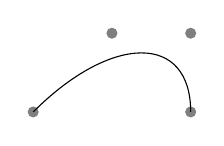
\begin{tikzpicture}
        \draw (0,0)..controls(1,1)and(2,1)..(2,0);%画曲线把--改为..,控制点至少有一个
        \foreach\x in{(0,0),(1,1),(2,1),(2,0)}\fill[black,opacity=0.5]\x circle(2pt);
      \end{tikzpicture}
    \mpics{0.7}
      \beginp{tikzpicture}\\
        \tbs{draw} (0,0)..controls(1,1)and(2,1)..(2,0);\\
        \tbs{foreach}\tbs{x} in{(0,0),(1,1),(2,1),(2,0)}\\
          \tbs{fill}[black,opacity=0.5]\tbs{x} circle(2pt);\\
      \pend{tikzpicture}
    \epics

    \bpics{0.4}
      
\begin{tikzpicture}[scale=.5]
        \draw[line width=4pt] (0,0) to [out=90, in=180] (3,2)
          to [out=-90, in=90] (8,-2);
      \end{tikzpicture}
    \mpics{0.6}
      \beginp{tikzpicture}[scale=.5]\\
        \tbs{draw}[line width=4pt] (0,0) to [out=90, in=180] (3,2)\\
          to [out=-90, in=90] (8,-2);\\
    \epics

    \bpics{0.3}
      \tikz \draw (0,0) ellipse (2pc and 1pc);
    \mpics{0.7}
      \tbs{tikz} \tbs{draw} (0,0) ellipse (2pc and 1pc);
    \epics

    \bpics{0.3}
      \tikz \draw(0,0)arc(0:270:1.75pc and 1pc);
    \mpics{0.7}
      \tbs{tikz} \tbs{draw}(0,0)arc(0:270:1.75pc and 1pc);
    \epics

    \bpics{0.3}
      \tikz \draw[x=2pt,y=2pt] (0,0) parabola bend (4,16) (6,12);
    \mpics{0.7}
      \tbs{tikz} \tbs{draw}[x=2pt,y=2pt] (0,0) parabola bend (4,16) (6,12);
    \epics

    \bpics{0.3}
      \tikz \draw[x=3.14ex,y=2ex] (0,0) sin (1,1) cos (2,0) sin (3,-1) cos (4,0)
        (0,1) cos (1,0) sin (2,-1) cos (3,0) sin (4,1);
    \mpics{0.7}
      \tbs{tikz} \tbs{draw}[x=3.14ex,y=2ex] (0,0) sin (1,1) cos (2,0) sin (3,-1) cos (4,0)\\
        (0,1) cos (1,0) sin (2,-1) cos (3,0) sin (4,1);
    \epics

\section{特殊图形}
    \bpics{0.3}
      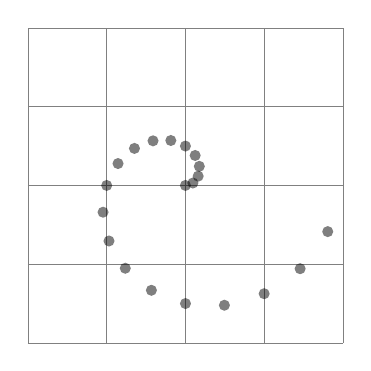
\begin{tikzpicture}
        \draw [help lines] (0,0) grid (4,4);
          \foreach \i in {0,0.1,...,2}
          \fill [black,opacity=0.5]($(2,2) !\i! \i*180:(3,2)$) circle (2pt);
      \end{tikzpicture}
    \mpics{0.7}
      \beginp{tikzpicture}\\
        \quad\tbs{draw} [help lines] (0,0) grid (4,4);\\
        \quad\tbs{foreach} \tbs{i} in {0,0.1,...,2}\\
          \qquad\tbs{fill} [black,opacity=0.5](\$(2,2) !\tbs{i}! \tbs{i}*180:(3,2)\$) circle (2pt);\\
      \pend{tikzpicture}
    \epics
\section{命令示例}
  \subsection{Plot}
    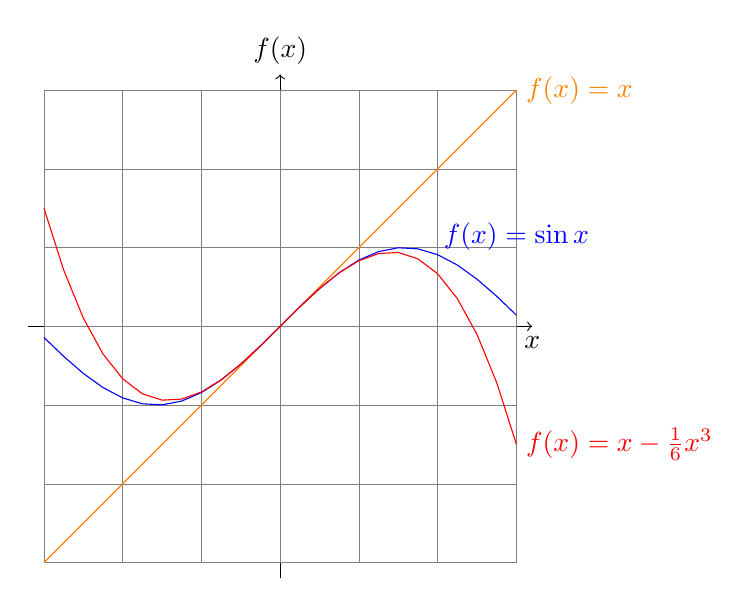
\begin{tikzpicture}[domain=-3:3]
      \draw[->] (-3.2,0) -- (3.2,0) node[below] {$x$};
      \draw[->] (0,-3.2) -- (0,3.2) node[above] {$f(x)$};
      \draw[very thin,color=gray] (-3,-3) grid (3,3);
      \draw[color=orange] plot (\x,\x) node[right] {$f(x)=x$};
      \draw[color=blue] plot (\x,{sin(\x r)}) node[above=7mm] {$f(x)=\sin x$};
      \draw[color=red] plot(\x,{\x-(1/6)*(\x)^3}) node[right]{$f(x)=x-\frac{1}{6}x^3$};
    \end{tikzpicture}

\begin{verbatim}
\begin{tikzpicture}[domain=-3:3]
\draw[->] (-3.2,0) -- (3.2,0) node[below] {$x$};
\draw[->] (0,-3.2) -- (0,3.2) node[above] {$f(x)$};
\draw[very thin,color=gray] (-3,-3) grid (3,3);
\draw[color=orange] plot (\x,\x) node[right] {$f(x)=x$};
\draw[color=blue] plot (\x,{sin(\x r)})
  node[above=7mm] {$f(x)=\sin x$};
\draw[color=red] plot(\x,{\x-(1/6)*(\x)^3})
  node[right]{$f(x)=x-\frac{1}{6}x^3$};
\end{verbatim}


  \subsection{Shading}
      \bpics{0.3}
        \tikz \shade (0,0) rectangle (2,1) (3,0.5) circle (0.5);
      \mpics{0.7}
        \tbs{tikz} \tbs{shade} (0,0) rectangle (2,1) (3,0.5) circle (0.5);
      \epics

      \bpics{0.4}
        \begin{tikzpicture}[rounded corners,ultra thick]
          \shade[top color=yellow,bottom color=black] (0,0) rectangle +(2,1);
          \shade[left color=yellow,right color=black] (3,0) rectangle +(2,1);
          \shadedraw[inner color=yellow,outer color=black,draw=yellow] (0,-1.5) rectangle +(2,1);
          \shade[ball color=green] (3.5,-1) circle(.5cm);
        \end{tikzpicture}
      \mpics{0.6}
        \beginp{tikzpicture}[rounded corners,ultra thick]\\
        \tbs{shade}[top color=yellow,bottom color=black]\\
          \quad(0,0) rectangle +(2,1);\\
        \tbs{shade}[left color=yellow,right color=black]\\
          \quad (3,0) rectangle +(2,1);\\
        \tbs{shadedraw}[inner color=yellow,outer color=black,draw=yellow]\\
          \quad(6,0) rectangle +(2,1);\\
        \tbs{shade}[ball color=green] (9,.5) circle(.5cm);
      \epics
  \subsection{XYZ}
      \bpics{0.3}
        \begin{tikzpicture}[->]
          \draw (0,0) -- (xyz cs:x=1);
          \draw (0,0) -- (xyz cs:y=1);
          \draw (0,0) -- (xyz cs:z=1);
        \end{tikzpicture}
      \mpics{0.7}
        \beginp{tikzpicture}[->]\\
          \tbs{draw} (0,0) -- (xyz cs:x=1);\\
          \tbs{draw} (0,0) -- (xyz cs:y=1);\\
          \tbs{draw} (0,0) -- (xyz cs:z=1);\\
      \epics

      \bpics{0.3}
        \tikz\node{root}child{node{left}}child{node{right}child{node{child}}child{node{child}}};
      \mpics{0.7}
        \tbs{tikz}\tbs{node}{root}\\
          child {node {left}}\\
          child {node {right}\\
          child {node {child}}\\
          child {node {child}}\\
          };
      \epics
  \subsection{scope}
      \bpics{0.4}
        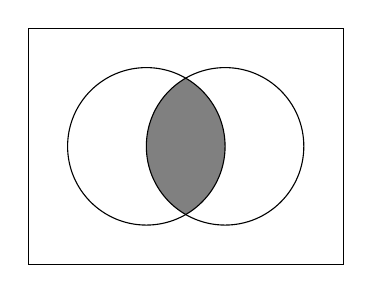
\begin{tikzpicture}
          \draw (-2, 1.5) rectangle (2, -1.5);
          \begin{scope}
            \clip (-0.5, 0) circle (1);
            \clip ( 0.5, 0) circle (1);
            \fill[color=gray] (-2,1.5)
              rectangle (2,-1.5);
          \end{scope}
          \draw (-0.5, 0) circle (1);
          \draw ( 0.5, 0) circle (1);
        \end{tikzpicture}
      \mpics{0.6}
      \beginp{tikzpicture}
          \tbs{draw} (-2, 1.5) rectangle (2, -1.5);
          \beginp{scope}
            \tbs{clip} (-0.5, 0) circle (1);
            \tbs{clip} ( 0.5, 0) circle (1);
            \tbs{fill}[color=gray] (-2,1.5)
              rectangle (2,-1.5);
          \pend{scope}
          \tbs{draw} (-0.5, 0) circle (1);
          \tbs{draw} ( 0.5, 0) circle (1);
         \pend{tikzpicture}
      \epics


  \subsection{even odd rule}
      \bpics{0.3}
        
\begin{tikzpicture}[even odd rule,rounded corners=2pt,x=10pt,y=10pt] %奇数有色,偶数无色
        \filldraw[fill=yellow!80!black] (0,0) rectangle (1,1)
          [xshift=5pt,yshift=5pt] (0,0) rectangle (1,1) %移动坐标
          [rotate=30] (-1,-1) rectangle (2,2); %先画好,再移动
        \end{tikzpicture}
      \mpics{0.7}
\begin{verbatim}

\begin{tikzpicture}[
  even odd rule,rounded corners=2pt,x=10pt,y=10pt]
\filldraw[fill=yellow!80!black] (0,0) rectangle (1,1)
[xshift=5pt,yshift=5pt] (0,0) rectangle (1,1)
[rotate=30] (-1,-1) rectangle (2,2);
\end{tikzpicture}
\end{verbatim}
      \epics

  \subsection{Foreach}
      \bpics{0.3}
        \foreach \x in{1,2,3} {$x=\x$, }
      \mpics{0.7}
        \tbs{foreach} \tbs{x} in\{1,2,3\} \{\$x=\tbs{x}\$, \}
      \epics


        \tikz \foreach \x in {1,...,5} \draw (\x,0) circle (0.4);

        \verb|\tikz \foreach \x in {1,...,10} \draw (\x,0) circle (0.4);|

      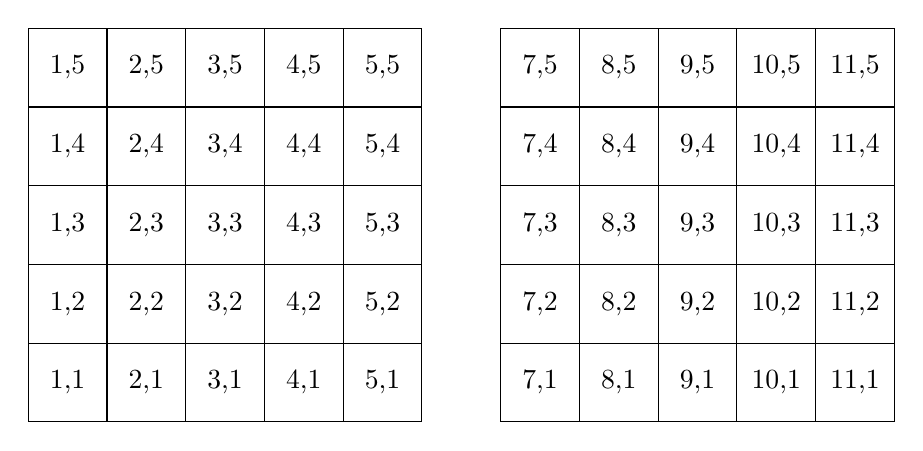
\begin{tikzpicture}
        \foreach \x in {1,2,...,5,7,8,...,11}
          \foreach \y in {1,...,5}
            { \draw (\x,\y) +(-.5,-.5) rectangle ++(.5,.5);
        \draw (\x,\y) node{\x,\y}; }
      \end{tikzpicture}

    \begin{verbatim}
    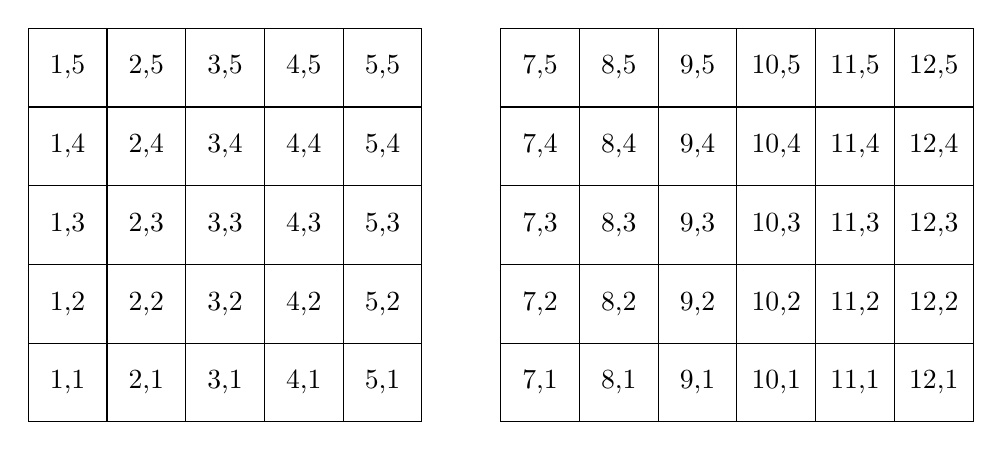
\begin{tikzpicture}
    \foreach \x in {1,2,...,5,7,8,...,12}
    \foreach \y in {1,...,5}
    { \draw (\x,\y) +(-.5,-.5)
      rectangle +(.5,.5);
    \draw (\x,\y) node{\x,\y}; }
    \end{tikzpicture}
    \end{verbatim}


  \subsection{Node}
      node 命令的可选项 left , right , above , below 用于控制插入文本的位置。此外还有 above right , below right , above left ,below left 等。\sky
      文本对齐用 align=left , align=right , align=center 来控制\sky
      在 node 里面用 includegraphics 命令可以插入图片\sky

      \bpics{0.3}
        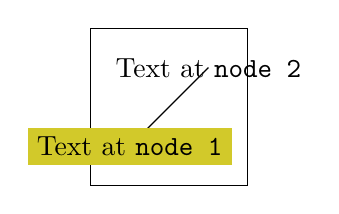
\begin{tikzpicture}
          \draw (0,0) rectangle (2,2);
          \draw (.5,.5) node[fill=yellow!80!black]{Text at \verb|node 1|}
            --(1.5,1.5) node{Text at \verb|node 2|};
        \end{tikzpicture}
      \mpics{0.7}
        \beginp{tikzpicture}
          \tbs{draw} (0,0) rectangle (2,2);
          \tbs{draw} (.5,.5) node[fill=yellow!80!black]{Text at \verb|node 1|}
            \quad--(1.5,1.5) node{Text at \verb|node 2|};
      \epics

      \bpics{0.4}
        \begin{tikzpicture}
          \draw[->] (-2.2,0)--(3.4,0);
          \foreach \x/\xtext in {-2,-1,1,2} \draw (\x,0pt)--(\x,2pt) node[near start,below]{$\xtext$};
          \draw[->] (0,-2.3)--(0,2.4);
          \foreach \y in {-2,-1,1,2} \draw (0pt,\y)--(2pt,\y) node[near start,left]{$\y$};
          \draw (0,0) node[very near start,below left]{$0$};
        \end{tikzpicture}
      \mpics{0.6}
        \beginp{tikzpicture}
          \tbs{draw}[->] (-2.2,0)--(3.4,0);\\
          \tbs{foreach} \tbs{x}/\tbs{xtext} in \{-2,-1,1,2\} \\
            \quad\tbs{draw} (\tbs{x},0pt)--(\tbs{x},2pt) \\
            \quad node[near start,below]\{\$\tbs{xtext}\$\};\\
          \tbs{draw}[->] (0,-2.3)--(0,2.4);\\
          \tbs{foreach} \tbs{y} in \{-2,-1,1,2\}\\
            \quad\tbs{draw} (0pt,\tbs{y})--(2pt,\tbs{y})\\
            \quad node[near start,left]\{\$\tbs{y}\$\};\\
          \tbs{draw} (0,0) node[very near start,below left]\{\$0\$\};\\
        \pend{tikzpicture}
      \epics



\subsection{Style}
\begin{verbatim}
\tikzset{help lines/.style= {step=0.5cm,color=gray!40,very thin}}

\tikzset{style001/.style={color=red,fill=red!20}}
\tikzset{help lines/.append style=blue!50}%原样式修改

\tikz \path (top-left) ++(1,-2) coordinate (name-point);%定义相对点

这种形式 (p1 |- xline) 表示取第一个点的 x 和第二个点的 y 组成一个新的点。
如果是 (p1 -| xline) 表示取第二个点的 x 和第一个点的 y 组成一个新的点。

shorten >=-0.4cm,shorten <=-0.4cm
可以通过类似上面的选项让两个点确定的线条延长,
不过这种延长是不能用 intersection 方法处理的。
其中 >= 表示到第二个点超过
的部分,负值表示超过;然后 <= 表示到第一个点超过的部分,正值则缩回去了。
\end{verbatim}
\section{实例}
\subsection{三角函数}
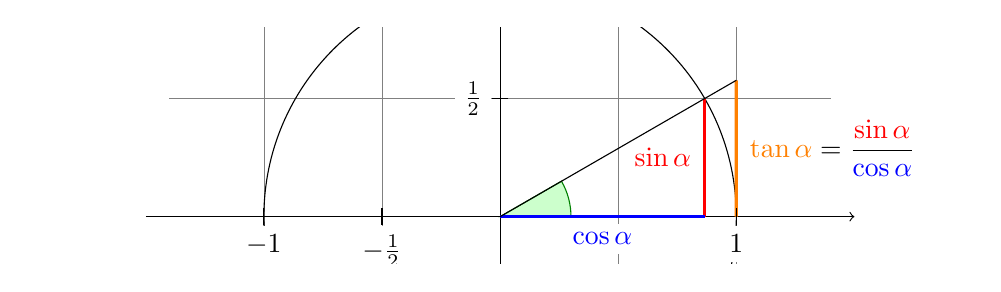
\begin{tikzpicture}[scale=3]
\clip (-2,-0.2) rectangle (2,0.8);
\draw[step=.5cm,gray,very thin] (-1.4,-1.4) grid (1.4,1.4);
\filldraw[fill=green!20,draw=green!50!black] (0,0) -- (3mm,0mm)
arc [start angle=0, end angle=30, radius=3mm] -- cycle;
\draw[->] (-1.5,0) -- (1.5,0) coordinate (x axis);
\draw[->] (0,-1.5) -- (0,1.5) coordinate (y axis);
\draw (0,0) circle [radius=1cm];
\draw[very thick,red]
(30:1cm) -- node[left=1pt,fill=white]{$\sin \alpha$} (30:1cm |- x axis);
\draw[very thick,blue]
(30:1cm |- x axis) -- node[below=2pt,fill=white] {$\cos \alpha$} (0,0);
\path [name path=upward line] (1,0) -- (1,1);
\path [name path=sloped line] (0,0) -- (30:1.5cm);
\draw [name intersections={of=upward line and sloped line, by=t}]
[very thick,orange] (1,0) -- node [right=1pt,fill=white]
{$\displaystyle \tan \alpha \color{black}=
\frac{{\color{red}\sin \alpha}}{\color{blue}\cos \alpha}$} (t);
\draw (0,0) -- (t);
\foreach \x/\xtext in {-1, -0.5/-\frac{1}{2}, 1}
\draw (\x cm,1pt) -- (\x cm,-1pt) node[anchor=north,fill=white] {$\xtext$};
\foreach \y/\ytext in {-1, -0.5/-\frac{1}{2}, 0.5/\frac{1}{2}, 1}
\draw (1pt,\y cm) -- (-1pt,\y cm) node[anchor=east,fill=white] {$\ytext$};
\end{tikzpicture}

\begin{verbatim}
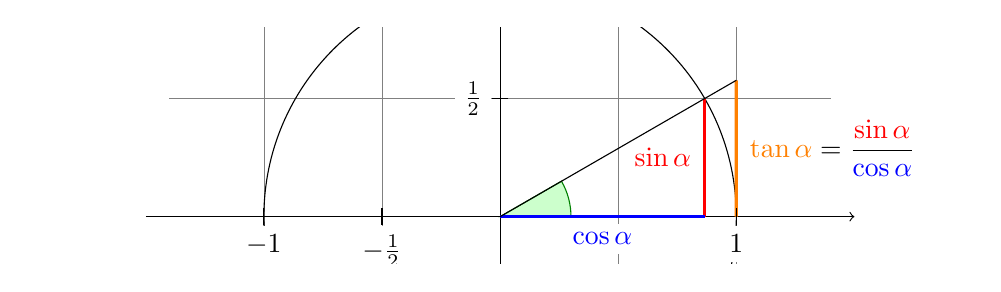
\begin{tikzpicture}[scale=3]
\clip (-2,-0.2) rectangle (2,0.8); %设定画图范围
\draw[step=.5cm,gray,very thin] (-1.4,-1.4) grid (1.4,1.4);
\filldraw[fill=green!20,draw=green!50!black] (0,0) -- (3mm,0mm)
arc [start angle=0, end angle=30, radius=3mm] -- cycle;
\draw[->] (-1.5,0) -- (1.5,0) coordinate (x axis);
\draw[->] (0,-1.5) -- (0,1.5) coordinate (y axis);
\draw (0,0) circle [radius=1cm];
\draw[very thick,red]
(30:1cm) -- node[left=1pt,fill=white] {$\sin \alpha$}
(30:1cm |- x axis); %|-表示画垂线
\draw[very thick,blue]
(30:1cm |- x axis) -- node[below=2pt,fill=white] {$\cos \alpha$} (0,0);
\path [name path=upward line] (1,0) -- (1,1); % 命名路径
\path [name path=sloped line] (0,0) -- (30:1.5cm);
\draw [name intersections={of=upward line and sloped line, by=t}] %交点
[very thick,orange] (1,0) --
node [right=1pt,fill=white]
{$\displaystyle\tan\alpha\color{black}=
  \frac{{\color{red}\sin\alpha}}{\color{blue}\cos\alpha}$}(t);
\draw (0,0) -- (t);
\foreach \x/\xtext in {-1, -0.5/-\frac{1}{2}, 1}%注意1/2的表示法
\draw (\x cm,1pt) -- (\x cm,-1pt) node[anchor=north,fill=white] {$\xtext$};
\foreach \y/\ytext in {-1, -0.5/-\frac{1}{2}, 0.5/\frac{1}{2}, 1}
\draw (1pt,\y cm) -- (-1pt,\y cm) node[anchor=east,fill=white] {$\ytext$};
\end{tikzpicture}
\end{verbatim}

\subsection{等边三角形}
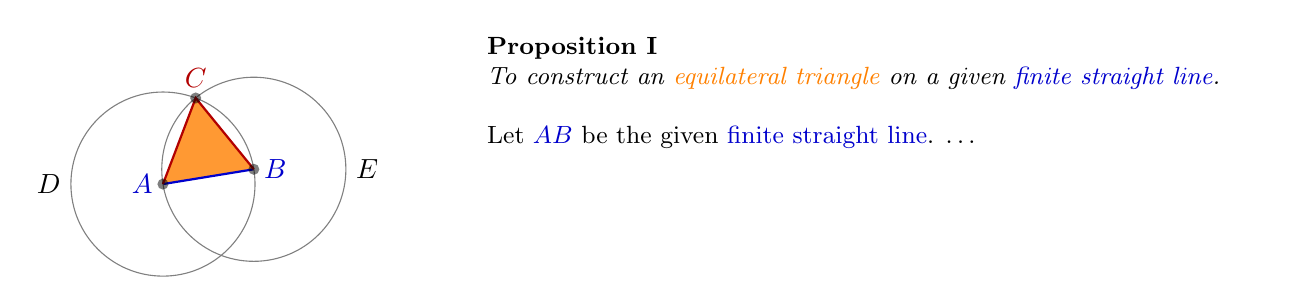
\begin{tikzpicture}[thick]
\tikzset{help lines/.style={thin,draw=black!50}}
\def\A{\textcolor{input}{$A$}}  \def\B{\textcolor{input}{$B$}}
\def\C{\textcolor{output}{$C$}}
\colorlet{input}{blue!80!black} \colorlet{output}{red!70!black}
\colorlet{triangle}{orange}

\coordinate[label=left:\A](A)at($(0,0)+.1*(rand,rand)$);
\coordinate[label=right:\B](B)at($(1.25,0.25)+.1*(rand,rand)$);
\draw [input](A)--(B);
\node[name path=D,help lines,draw,label=left:\D](D)at(A)[circle through=(B)]{};
\node[name path=E,help lines,draw,label=right:\E](E)at(B)[circle through=(A)]{};
\path[name  intersections={of=D and E,by={[label=above:\C]C}}];
\draw[output](A)--(C)--(B);
\foreach \point in {A,B,C}\fill[black,opacity=.5](\point)circle(2pt);

\begin{pgfonlayer}{background}
\fill[triangle!80] (A) -- (C) -- (B) -- cycle;
\end{pgfonlayer}

\node [below right, text width=10cm,align=justify] at (4,2) {
\small\textbf{Proposition I}\par
\emph{To construct an \textcolor{triangle}{equilateral triangle}
on a given \textcolor{input}{finite straight line}.}
\par\vskip1em
Let \A\B\ be the given \textcolor{input}{finite straight line}. \dots
};
\end{tikzpicture}
\begin{verbatim}
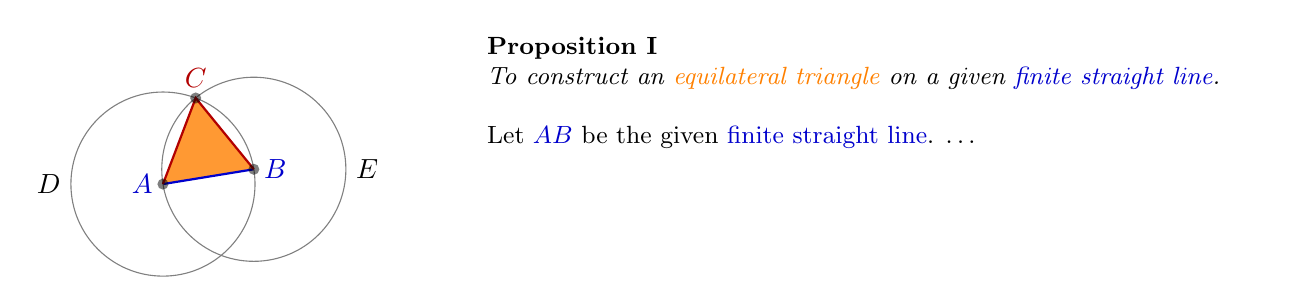
\begin{tikzpicture}[thick]
\tikzset{help lines/.style={thin,draw=black!50}}
\def\A{\textcolor{input}{$A$}}  \def\B{\textcolor{input}{$B$}}
\def\C{\textcolor{output}{$C$}} \def\D{$D$}  \def\E{$E$}
\colorlet{input}{blue!80!black} \colorlet{output}{red!70!black}
\colorlet{triangle}{orange}

\coordinate[label=left:\A](A)at($(0,0)+.1*(rand,rand)$);
\coordinate[label=right:\B](B)at($(1.25,0.25)+.1*(rand,rand)$);
\draw [input](A)--(B);
\node[name path=D,help lines,draw,label=left:\D](D)at(A)[circle through=(B)]{};
\node[name path=E,help lines,draw,label=right:\E](E)at(B)[circle through=(A)]{};
\path[name  intersections={of=D and E,by={[label=above:\C]C}}];
\draw[output](A)--(C)--(B);
\foreach \point in {A,B,C}\fill[black,opacity=.5](\point)circle(2pt);

\begin{pgfonlayer}{background}
\fill[triangle!80] (A) -- (C) -- (B) -- cycle;
\end{pgfonlayer}

\node [below right, text width=10cm,align=justify] at (4,2) {
\small\textbf{Proposition I}\par
\emph{To construct an \textcolor{triangle}{equilateral triangle}
on a given \textcolor{input}{finite straight line}.}
\par\vskip1em
Let \A\B\ be the given \textcolor{input}{finite straight line}. \dots
};
\end{tikzpicture}
\end{verbatim}


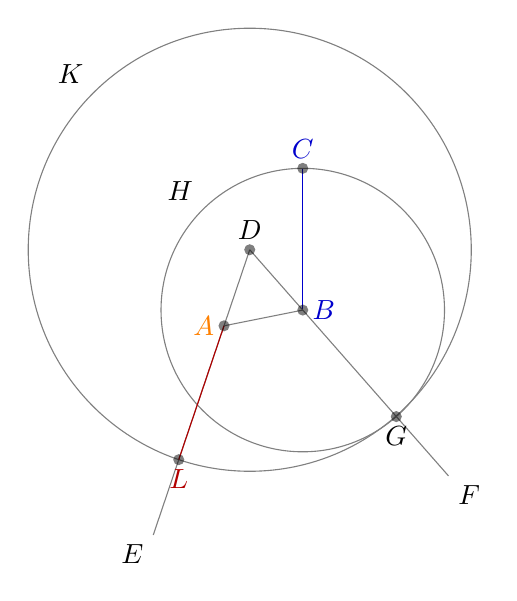
\begin{tikzpicture}
\tikzset{help lines/.style={thin,draw=black!50}}
\def\A{\textcolor{orange}{$A$}} \def\B{\textcolor{input}{$B$}}
\def\C{\textcolor{input}{$C$}}  \def\L{\textcolor{output}{$L$}}
\colorlet{input}{blue!80!black} \colorlet{output}{red!70!black}

\coordinate[label=left:\A](A)at(0,0);
\coordinate[label=right:\B](B)at(1,0.2);
\coordinate[label=above:\C](C)at(1,2);
\draw[input](B)--(C);
\draw[help lines](A)--(B);
\coordinate[label=above:\D](D)at($(A)!.5!(B)!{sin(60)*2}!90:(B)$);

\draw[help lines](D)--($(D)!3.75!(A)$) coordinate[label=-135:\E](E);
\draw[help lines](D)--($(D)!3.75!(B)$) coordinate[label=-45:\F](F);
\node[name path=H,help lines,circle through=(C),draw,label=135:\H](H)at(B){};

\path[name path=B--F](B)--(F);
\path[name intersections={of=H and B--F,by={[label=below:\G]G}}];
\node(K)at(D)[name path=K,help lines,circle through=(G),draw,label=135:\K]{};

\path[name path=A--E](A)--(E);
\path[name intersections={of=K and A--E,by={[label=below:\L]L}}];
\draw[output](A)--(L);

\foreach \point in {A,B,C,D,G,L}
\fill[black,opacity=.5](\point)circle(2pt);
\end{tikzpicture}
\begin{verbatim}
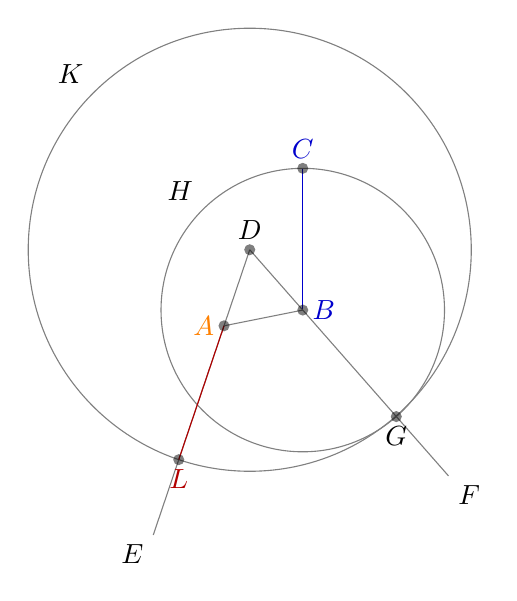
\begin{tikzpicture}
\tikzset{help lines/.style={thin,draw=black!50}}
\def\A{\textcolor{orange}{$A$}} \def\B{\textcolor{input}{$B$}}
\def\C{\textcolor{input}{$C$}}  \def\L{\textcolor{output}{$L$}}
\colorlet{input}{blue!80!black} \colorlet{output}{red!70!black}

\coordinate[label=left:\A](A)at(0,0);
\coordinate[label=right:\B](B)at(1,0.2);
\coordinate[label=above:\C](C)at(1,2);
\draw[input](B)--(C);
\draw[help lines](A)--(B);
\coordinate[label=above:\D](D)at($(A)!.5!(B)!{sin(60)*2}!90:(B)$);

\draw[help lines](D)--($(D)!3.75!(A)$) coordinate[label=-135:\E](E);
\draw[help lines](D)--($(D)!3.75!(B)$) coordinate[label=-45:\F](F);
\node[name path=H,help lines,circle through=(C),draw,label=135:\H](H)at(B){};

\path[name path=B--F](B)--(F);
\path[name intersections={of=H and B--F,by={[label=below:\G]G}}];
\node(K)at(D)[name path=K,help lines,circle through=(G),draw,label=135:\K]{};

\path[name path=A--E](A)--(E);
\path[name intersections={of=K and A--E,by={[label=below:\L]L}}];
\draw[output](A)--(L);

\foreach \point in {A,B,C,D,G,L}
\fill[black,opacity=.5](\point)circle(2pt);
\end{tikzpicture}
\end{verbatim}


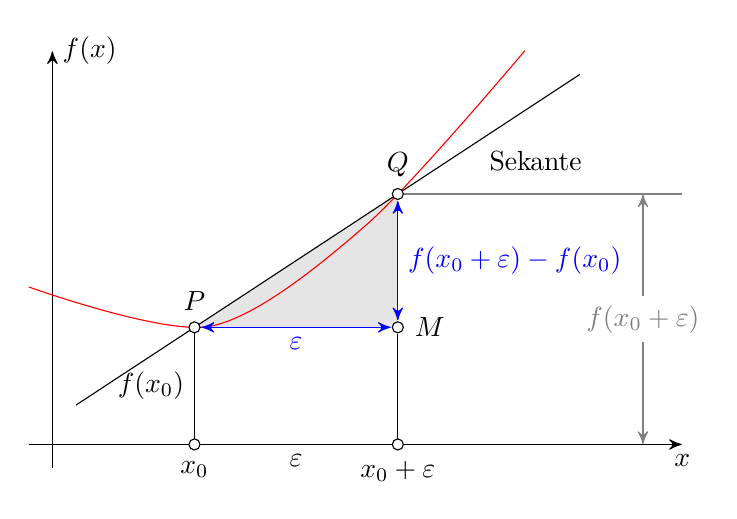
\begin{tikzpicture}
\tikzset{thick,>=stealth',dot/.style={draw,fill=white,circle,inner sep=0pt,minimum size=4pt}}
\coordinate (O) at (0,0);
\draw[->] (-0.3,0)--(8,0) coordinate[label={below:$x$}] (xmax);
\draw[->] (0,-0.3)--(0,5) coordinate[label={right:$f(x)$}] (ymax);
\path[name path=x] (0.3,0.5) -- (6.7,4.7);
\path[name path=y] plot[smooth] coordinates {(-0.3,2) (2,1.5) (4,2.8) (6,5)};

\begin{scope}[name intersections = {of= x and y,name = i}]
\fill[gray!20] (i-1) -- (i-2 |- i-1) -- (i-2) -- cycle;
\draw (0.3,0.5) -- (6.7,4.7) node[pos=0.8,below right] {Sekante};
\draw[red] plot[smooth] coordinates {(-0.3,2) (2,1.5) (4,2.8) (6,5)};
\draw (i-1) node[dot,label={above:$P$}] (i-1) {} -- node[left] {$f(x_0)$} (i-1 |- O) node[dot,label={below:$x_0$}] {};
\path (i-2) node[dot,label={above:$Q$}] (i-2) {} -- (i-2 |- i-1) node[dot,label={right:$M$}] (i-12) {};
\draw (i-12) -- (i-12 |- O) node[dot,label={below:$x_0 + \varepsilon$}] {};
\draw[blue,<->] (i-2) -- node[right] {$f(x_0 + \varepsilon) - f(x_0)$} (i-12);
\draw[blue,<->] (i-1) -- node[below] {$\varepsilon$} (i-12);
\path (i-1 |- O) -- node[below] {$\varepsilon$} (i-2 |- O);
\draw[gray] (i-2) -- (i-2 -| xmax);
\draw[gray,<->] ([xshift=-0.5cm]i-2 -| xmax) -- node[fill=white] {$f(x_0 + \varepsilon)$}  ([xshift=-0.5cm]xmax);
\end{scope}

\end{tikzpicture}
\begin{verbatim}
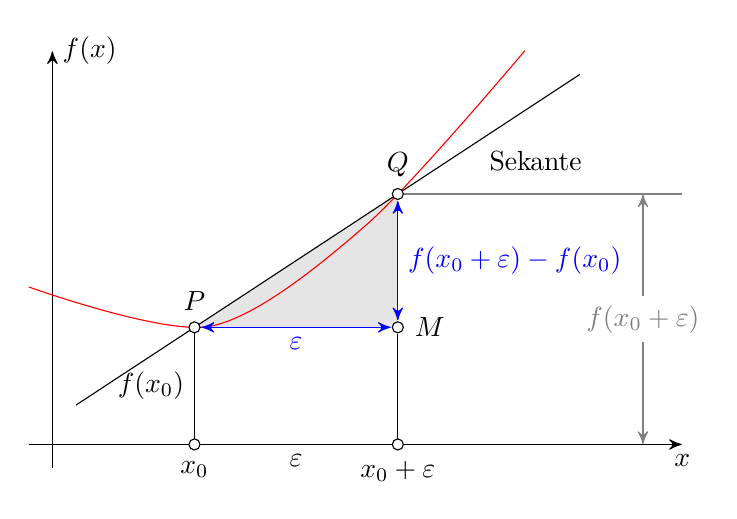
\begin{tikzpicture}
\tikzset{thick,>=stealth',dot/.style={draw,fill=white,circle,inner sep=0pt,minimum size=4pt}}
\coordinate (O) at (0,0);
\draw[->] (-0.3,0)--(8,0) coordinate[label={below:$x$}] (xmax);
\draw[->] (0,-0.3)--(0,5) coordinate[label={right:$f(x)$}] (ymax);
\path[name path=x] (0.3,0.5) -- (6.7,4.7);
\path[name path=y] plot[smooth] coordinates {(-0.3,2) (2,1.5) (4,2.8) (6,5)};
\begin{scope}[name intersections = {of= x and y,name = i}]
\fill[gray!20] (i-1) -- (i-2 |- i-1) -- (i-2) -- cycle;
\draw (0.3,0.5) -- (6.7,4.7) node[pos=0.8,below right] {Sekante};
\draw[red] plot[smooth] coordinates {(-0.3,2) (2,1.5) (4,2.8) (6,5)};
\draw (i-1) node[dot,label={above:$P$}] (i-1) {} -- node[left] {$f(x_0)$} (i-1 |- O) node[dot,label={below:$x_0$}] {};
\path (i-2) node[dot,label={above:$Q$}] (i-2) {} -- (i-2 |- i-1) node[dot,label={right:$M$}] (i-12) {};
\draw (i-12) -- (i-12 |- O) node[dot,label={below:$x_0 + \varepsilon$}] {};
\draw[blue,<->] (i-2) -- node[right] {$f(x_0 + \varepsilon) - f(x_0)$} (i-12);
\draw[blue,<->] (i-1) -- node[below] {$\varepsilon$} (i-12);
\path (i-1 |- O) -- node[below] {$\varepsilon$} (i-2 |- O);
\draw[gray] (i-2) -- (i-2 -| xmax);
\draw[gray,<->] ([xshift=-0.5cm]i-2 -| xmax) -- node[fill=white] {$f(x_0 + \varepsilon)$}  ([xshift=-0.5cm]xmax);
\end{scope}
\end{tikzpicture}
\end{verbatim}

\section{Library}
    \subsection{Angels}
      \bpics{0.3}
        \tikz \draw (2,0) coordinate(A)--(0,0)coordinate(B)--(-1,-1)coordinate(C)
          pic [fill=black!50] {angle = A--B--C}
          pic [draw,->,red,thick,angle radius=1cm] {angle = C--B--A};
      \mpics{0.7}
\begin{verbatim}
\tikz \draw (2,0) coordinate(A)--(0,0)coordinate(B)--(-1,-1)coordinate(C)
pic [fill=black!50] {angle = A--B--C}
pic [draw,->,red,thick,angle radius=1cm] {angle = C--B--A};
\end{verbatim}
      \epics

\subsection{Math}
\tikzmath{function fibonacci(\n){
if \n == 0 then {return 0;}
else {return fibonacci2(\n, 0, 1);};
};
function fibonacci2(\n, \p, \q){
if \n == 1 then {return \q;}
else {return fibonacci2(\n-1, \q, \p+\q);};
};
int \f, \i;
for \i in {0,1,...,20}{\f= fibonacci(\i); print {\f,};
};}
\begin{verbatim}
\tikzmath{function fibonacci(\n){
if \n == 0 then {return 0;}
else {return fibonacci2(\n, 0, 1);};
};
function fibonacci2(\n, \p, \q){
if \n == 1 then {return \q;}
else {return fibonacci2(\n-1, \q, \p+\q);};
};
int \f, \i;
for \i in {0,1,...,20}{\f= fibonacci(\i); print {\f,};
};}
\end{verbatim}\sky

      \bpics{0.3}
        \tikz[x=0.25cm,y=0.25cm,evaluate={
          int \i, \j;
        for \i in {0,...,10}{
          for \j in {0,...,10}{
            \a{\i,\j} = (\i+\j)*5;};};}]
        \foreach \i in {0,...,10}
          \foreach \j in {0,...,10}
            \fill [red!\a{\i,\j}!yellow] (\i,\j) rectangle ++(1, 1);
      \mpics{0.7}
\begin{verbatim}
\tikz[x=0.25cm,y=0.25cm,evaluate={
int \i, \j;
for \i in {0,...,10}{
for \j in {0,...,10}{
\a{\i,\j} = (\i+\j)*5;};};}]
\foreach \i in {0,...,10}
\foreach \j in {0,...,10}
\fill [red!\a{\i,\j}!yellow] (\i,\j) rectangle ++(1, 1);
\end{verbatim}
      \epics

\tikzmath{ int \x, \y, \z;
\x=random(2,5);
for \y in {0,...,6}{\z=\x^\y; print{$\x^\y=\z$,};};}
\begin{verbatim}
\tikzmath{ int \x, \y, \z;
\x=random(2,5);
for \y in {0,...,6}{\z=\x^\y; print{$\x^\y=\z$,};};}
\end{verbatim}\sky


  \subsection{backgrounds}
      \bpics{0.3}
        
\begin{tikzpicture}[ scale=.8,background rectangle/.style=
          {draw=blue!50,fill=blue!20,rounded corners=1ex},show background rectangle]%show background grid
        \draw (2,2) circle (1);
        \draw (1 mm, 10 pt) -- (4 em, 1);
        \end{tikzpicture}
      \mpics{0.7}
\begin{verbatim}
\begin{tikzpicture}[ scale=.8,background rectangle/.style=
{draw=blue!50,fill=blue!20,rounded corners=1ex},show background rectangle]
\draw (2,2) circle (1);
\draw (1 mm, 10 pt) -- (4 em, 1);
\end{verbatim}
      \epics

\subsection{shapes}

\begin{tikzpicture}
\node[circle,draw]at(0,4){circle};
\node[star,draw]at(2,4){star};
\node[rectangle,draw]at(4,4){rectangle};
\node[diamond,draw]at(6,4){diamond};
\node[trapezium,trapezium left angle=75, trapezium right angle=45,draw]at(8,4){trapezium};
\node[semicircle,draw]at(10,4){semicircle};
\node[regular polygon,regular polygon sides=5,draw]at(13,4){regular polygon};
\node[regular polygon,regular polygon sides=7,minimum size=1cm,draw]at(0,2){};
\node[ellipse,draw]at(2,2){ellipse};
\node[kite,draw]at(4,2){kite};
\node[dart,draw, shape border uses incircle,shape border rotate=45]at(6,2){dart};
\end{tikzpicture}

\section{变换}
xscale=-1 或者 yscale=-1 就刚好相对 y 轴或 x 轴反对称。
\end{document} 
